\entry{Semana del 06/10/2025.} 

\section{Lunes 06/10/2025.} 

estaba viendo alternativas para calcular los exponentes y las frecuencias de corte.  Una cosa para revisar puede ser el análisis de Wavelets, que termina dando un espectro de energía como el que se ve acá abajo. 

\begin{figure}[th!]
	\centering
	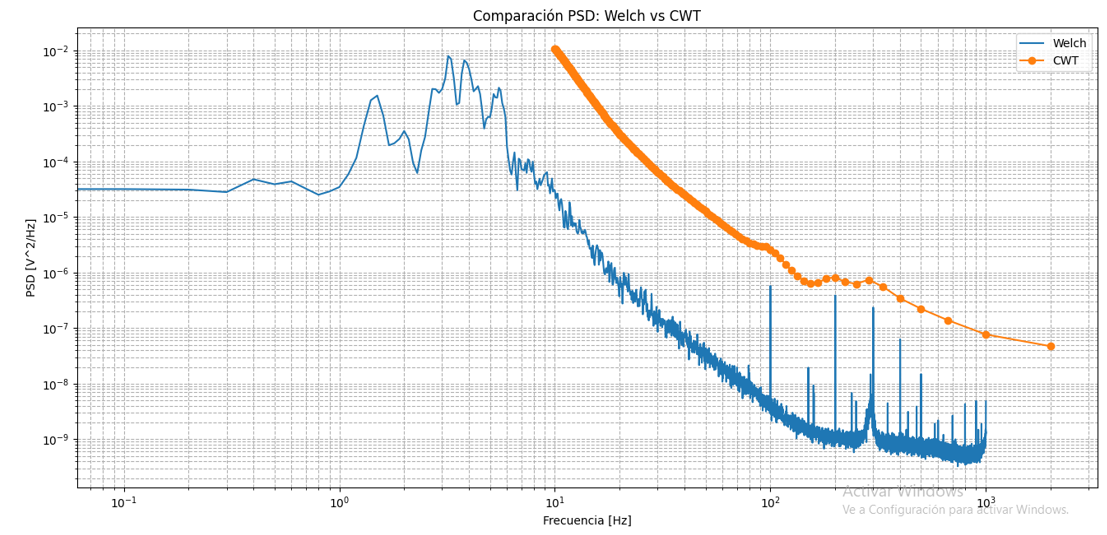
\includegraphics[width=0.5617\linewidth]{Figures/06_10_2025/CWT_0_6_Hz}
	\caption{Comparación de CWT con Welch para la medición de 0 a 6 Hz.}
	\label{fig:cwt06hz}
\end{figure}

Tarda un tiempo varios órdenes de magnitud mayor a lo que tarda Welch y suaviza un poco raro los picos en 50 Hz, 100 Hz, etc... Más allá de eso da un espectro super suave, pero todavía no entiendo bien qué son los Wavelets, solo que se supone que al usar paquetes en vez de senos y cosenos que serían finitos funciona mejor para señales reales.   

Wavelet vendría a ser una especie de Fourier por ventanas. Habría que revisar el periodograma que tira directamente, ya que eso va a dar una definición natural de qué escalas usar. Se pueden probar usar otras wavelets para ver si saca los picos de ruido (en la Figura estaba Morlet). 

\subsection*{Derivada logarítmica para exponentes.} 
Estuve charlando con Julián para usar la derivada logarítmica como parámetro para hallar los exponentes del espectro. Básicamente el método consiste en separar el espectro en ventanas de frecuencias e ir ajustando esas ventanas. Después hacemos eso mismo para cada espectro (de cada ventana temporal) y hacemos un histograma con todos esos exponentes esperando tener un pico en los exponentes que tendrá el espectro. 


\begin{figure}[th!]
	\centering
	\includegraphics[width=0.708\linewidth]{"Figures/06_10_2025/Derivada logarítmica"}
	\caption{Derivada logarítmica de los espectros de la serie de 0 a 6 Hz con ventana temporal de 1 s y en frecuencia de 10  Hz.}
	\label{fig:derivada-logaritmica}
\end{figure}

Lo único que no termina de convencer, por lo menos con los parámetros que probé, es que necesito ventanas para ajustar bastante grandes, y de por sí suavizar el espectro.  
 
 
 